\section{Evaluation}
    \subsection{Evaluation Critera}
        \begin{frame}
            \frametitle{Evaluation}
            \begin{itemize}
                \item Applicability
                    \begin{itemize}
                        \item our claim is that MSR tasks and hypotheses can be ex- pressed and evaluated using Candoia platform\'s capabilities.
                    \end{itemize}
                \item Adoptability
                    \begin{itemize}
                        \item Candoia apps are portable across diverse project settings and require no changes
                    \end{itemize}
                \item Customizability
                    \begin{itemize}
                        \item Our claim that performing customizations in Candoia requires less efforts in terms of LOC.
                    \end{itemize}
            \end{itemize}
         \end{frame}

        \begin{frame}
            \frametitle{Projects used in Evaluation}
            \begin{figure}[ht!]
\centering
% Please add the following required packages to your document preamble:
% \usepackage[table,xcdraw]{xcolor}
% If you use beamer only pass "xcolor=table" option, i.e. \documentclass[xcolor=table]{beamer}
%\resizebox{0.99\textwidth}{!}{%
% \small
\begin{adjustbox}{max width=0.9\textwidth}
\begin{tabular}{|
>{\columncolor[HTML]{C0C0C0}}l |l|l|l|r|r|r|r|}
\hline
Projects        &
\multicolumn{1}{c|}{\cellcolor[HTML]{C0C0C0}VCS} &
\multicolumn{1}{c|}{\cellcolor[HTML]{C0C0C0}PL}   &
\multicolumn{1}{c|}{\cellcolor[HTML]{C0C0C0}Bugs} &
\multicolumn{1}{c|}{\cellcolor[HTML]{C0C0C0}\#LOC} & 
\multicolumn{1}{c|}{\cellcolor[HTML]{C0C0C0}\#Revs} & 
\multicolumn{1}{c|}{\cellcolor[HTML]{C0C0C0}\#Bugs} & 
\multicolumn{1}{c|}{\cellcolor[HTML]{C0C0C0}\#Devs} \\
\hline 
Tomcat 8.0.24 (TC)  & SVN  & Java  & Bugzilla & 381350 & 17433 & 3023 & 32 \\
\hline

Hadoop 2.7.1 (HD)   & Git  & Java  & JIRA     & 2217636 & 14301 & 10333 & 146 \\ \hline

JUnit 4  (JU)       &Git   & Java  & GitHub   & 30535  & 2115  & 148  & 127 \\ \hline

SLF4j 1.7.12 (SLF)  & Git  & Java  & JIRA     & 20866  & 1436 & 332 & 59 \\ \hline

Bootstrap 3.3.5 (BT)& Git  & JS    & GitHub   & 65885 & 11840  & 213  & 718 \\
\hline

Node.js 0.12.7 (ND) & Git  & JS    & GitHub   & 3405739 & 14695   & 955 & 105 \\
\hline

Grunt 0.4.6  (GT)   & Git  & JS    & GitHub   & 3596 & 1399 & 155 & 29 \\ \hline

JQuery 2.1.4 (JQ)   & Git  & JS    & GitHub   & 45212  & 6153  & 165  & 87 \\
\hline

PMD 5.3.3 (PMD)     & Git  & Java  & SF       & 175866  & 8736  & 1394  & 102 \\
\hline

JEdit 5.2.0 (JE)    & SVN  & Java  & SF       & 224127  & 24509  & 3926  & 7 \\
\hline
\end{tabular}
\end{adjustbox}
%}
\caption{Test projects.}
\label{tab:projects}
\end{figure}

         \end{frame}

    \subsection{Applicability}
        \begin{frame}
            \frametitle{Applicability}
                \textbf{Claim:} MSR tasks and hypotheses can be ex- pressed and evaluated using Candoia \\
             \textbf{Evaluation Strategy:}
            \begin{itemize}
                \item Created 24 Candoia apps covering
                \begin{itemize}
                    \item Bugs
                    \item Software Evolution
                    \item Project Management
                    \item Source code analysis and Programming practices
                \end{itemize}
                \item Tested these applications over test projects
            \end{itemize}
         \end{frame}

        \begin{frame}
            \frametitle{Candoia apps used in evaluation}
            % Please add the following required packages to your document preamble:
%\usepackage[table,xcdraw]{xcolor}
% If you use beamer only pass "xcolor=table" option, i.e. \documentclass[xcolor=table]{beamer}
%\usepackage[normalem]{ulem}
%\useunder{\uline}{\ul}{}
\begin{figure}
\centering
\resizebox{\textwidth}{!}{%
\begin{tabular}{|
>{\columncolor[HTML]{C0C0C0}}l
|l|c|c|c|c|c|r|r|r|r|r|r|r|r|r|r|}
\hline
%\# & \multicolumn{1}{c|}{\cellcolor[HTML]{C0C0C0}{\bf Candoia  App}}  & \multicolumn{5}{c|}{\cellcolor[HTML]{C0C0C0}{\bf Number of lines of code}}                                                                                                          & \multicolumn{10}{c|}{\cellcolor[HTML]{C0C0C0}{\bf Execution time (s)}}                                                                                                                                                                                                                                                              \\ \hline
\# & \multicolumn{1}{c|}{\cellcolor[HTML]{C0C0C0}{\bf Candoia  App}}  &
\multicolumn{5}{c|}{\cellcolor[HTML]{C0C0C0}{\bf Number of lines of code}}                                                                                                          & \multicolumn{10}{c|}{\cellcolor[HTML]{C0C0C0}{\bf Execution time (s)}}                                                                                                                                                                                                                                                              \\ \hline
   & \multicolumn{1}{c|}{\cellcolor[HTML]{C0C0C0}{\bf }}                                                                        & \cellcolor[HTML]{C0C0C0}Boa  & \cellcolor[HTML]{C0C0C0}JS  & \cellcolor[HTML]{C0C0C0}HTML  & \cellcolor[HTML]{C0C0C0}CSS &  \cellcolor[HTML]{C0C0C0}JSON                                                                          & \cellcolor[HTML]{C0C0C0}TC & \cellcolor[HTML]{C0C0C0}HD & \cellcolor[HTML]{C0C0C0}JU & \cellcolor[HTML]{C0C0C0}SLF & \cellcolor[HTML]{C0C0C0}BT  & \cellcolor[HTML]{C0C0C0}ND  & \cellcolor[HTML]{C0C0C0}GT & \cellcolor[HTML]{C0C0C0}JQ & \cellcolor[HTML]{C0C0C0}PMD & \cellcolor[HTML]{C0C0C0}JE \\ \hline

   & \multicolumn{1}{c|}{\cellcolor[HTML]{C0C0C0}{\bf I. Bugs}}                                                                &     &     &     &    &                 &                                &                                &                               &                               &                                   &                                &                               &                                &                             &                               \\ \hline
1  & Detects unreproducible or wont-fix bugs                             &44  &48   &38   &33   &16         & 30.6                          & 110.0                         & 5.9                          & 2.6                          & 40.5                             & 149.0                         & 2.1                          & 10.1                          & 20.6                       & 47.5                         \\ \hline
2  & Detects improper usage of null                            &45  &11   &25   &0   &16                                                   & 33.0                          & 152.0                         & 5.8                          & 3.5                          & 4.8                              & 26.3                           & 1.1                          & 3.3                           & 35.8                       & 89.4                         \\ \hline
3  & Detects improper use of double checked locking idiom                     &100  &6   &25   &32   &16                & 17.0                          & 74.0                          & 3.3                          & 1.6                          & 4.2                              & 24.4                           & 3.0                          & 1.1                           & 15.0                       & 55.4                         \\ \hline
4  & Detects improper usage of wait-notify idiom               &39  &52   &47   &32   &16                        & 8.1                           & 28.4                          & 2.3                          & 1.2                          & 2.5                              & 12.2                          & 1.8                          & 0.9                           & 8.9                        & 23.1                         \\ \hline
5  & Identifies fixing revisions that add null checks                 &98  &13   &43   &32   &16                               & 3.5                           & 8.1                           & 1.4                          & 2.1                          & 4.7                              & 23.4                          & 5.0                          & 1.4                           & 3.8                        & 5.2                          \\ \hline
   & \multicolumn{1}{c|}{\cellcolor[HTML]{C0C0C0}{\bf II. Software Evolution}}                                                                &     &     &     &    &                 &                                &                                &                               &                               &                                   &                                &                               &                                &                             &                               \\ \hline
6  & Lists most frequently changed files                       &08  &16   &43   &0   &16                                               & 28.7                          & 114.0                         & 5.9                          & 26.2                         & 35.7                              & 125.0                          & 2.2                          & 10.9                          & 19.1                       & 57.2                         \\ \hline
7  & Lists commits that involved a large number of files                            &10  &52   &47   &32   &16                          & 36.1                          & 124.0                         & 7.8                          & 4.0                          & 43.9                              & 108.0                         & 2.9                          & 12.5                          & 23.2                       & 48.9                         \\ \hline
8  & Commit blame assignment based on increase in repository size              &27  &52   &47   &32   &16                       & 60.9                          & 163.0                         & 9.8                          & 4.7                          & 62.0                             & 189.0                         & 3.2                          & 19.7                          & 32.5                       & 89.6                         \\ \hline
9  & Provides details of latest revision, e.g. total changed files etc.     &10  &52   &47   &32   &16      & 33.0                          & 95.1                          & 7.0                          & 3.1                          & 36.9                             & 100.0                         & 2.6                          & 12.2                          & 20.2                       & 48.12                         \\ \hline
10 & Provides details of developers' last commits              &55  &42   &41   &0   &16                                    & 42.7                          & 139.0                         & 11.8                          & 9.1                          & 48.1                             & 119.0                        & 8.25                          & 17.7                          & 28.4                       & 92.7                         \\ \hline
11 & Mining co-changed files via association mining & 20 & 12 & 34 & 0 & 16 & 11.2
& 7.9 & 7.3 & 7.8 & 10.2 & 46.8 & 0.1 & 9.2 & 9.4 & 86.4\\ \hline
12 & Compute churn rate for fixing bugs & 13 & 33 & 47 & 0 & 16 & 1.5 & 3.7
& 1.4 & 1.0 & 2.6 & 8.6 & 0.5 & 1.1 & 2.8 & 2.2 \\ \hline
   & \multicolumn{1}{c|}{\cellcolor[HTML]{C0C0C0}{\bf III. Project Management}}                                                          &     &     &     &    &                                    &                                &                                &                               &                               &                                   &                                &                               &                                &                             &                               \\ \hline
13 & Ranks developers by the number of commits                           &11
&52   &47   &32   &16                               & 31.7                           & 111.0                         & 5.4                          & 2.6                          & 42.2                             & 137.0                         & 2.5                          & 11.4                          & 22.0                       & 46.4                         \\ \hline

14 & Maps modules to developers &36  &48   &38   &33   &16      & 37.3
& 127.0                         & 7.2                          & 4.0                          & 46.5                             & 171.0                         & 2.5                          & 12.0                          & 24.8                       & 53.0                         \\ \hline

15 & Computes number of attributes (NOA)                        &17  &106   &36 
&0   &16                                                 & 5.0                           & 19.4                          & 1.8                          & 1.1                          & 2.3                              & 9.3                           & 0.7                          & 1.4                           & 5.5                        & 10.3                         \\ \hline

16 & Computes number of public methods (NPM)             &19  &106   &36   &0
&16                                                         & 1.1                           & 23.9                          & 2.1                          & 6.5                          & 2.2                              & 9.2                           & 0.7                          & 1.6                           & 6.1                        & 6.2                          \\ \hline

17 & Identifies developers writing empty or one word commit logs         &27 
&52   &47   &32   &16            & 31.3                          & 110.0                         & 6.4                          & 2.6                          & 35.8                             & 128.0                         & 2.4                          & 11.0                          & 35.0                       & 46.8                         \\ \hline

18 & Associate bugs and source files & 37 & 30 & 47 & 32 & 16 & 67.4 & 321.8
& 10.9 & 5.1 & 5.5 & 8.7 & 1.0 & 1.9 & 47.3 & 84.8 \\ \hline

   & \multicolumn{1}{c|}{\cellcolor[HTML]{C0C0C0}{\bf IV. Program analysis}}                                                         &     &     &     &    &           &                                &                                &                               &                               &                                   &                                &                               &                                &                             &                               \\ \hline

19 & Detects violation of naming conventions         &48  &48   &38   &33   &16 
& 10.7                          & 37.9                          & 0.7                          & 1.8                          & 2.5                              & 18.4                          & 1.2                          & 0.4                           & 15.3                       & 22.8                         \\ \hline

20 & Checks serialization-related properties              &51  &51   &47   &32  
 &16                       & 7.6                           & 23.3                          & 3.5                          & 1.5                          & 2.6                              & 9.6                           & 0.8                          & 1.7                           & 33                       & 17                         \\ \hline

21 & Detects static fields which are public but not final               &44  &48 
 &38   &33   &16          & 7.4                           & 28.7                          & 2.9                          & 1.3                          & 2.6                              & 10.0                           & 0.7                          & 1.5                           & 9.4                        & 15.7                         \\ \hline

22 & Identifies locations of dead code                                     &47 
 &52   &47   &32   &16                                    & 18.2                          & 110.0                         & 4.8                          & 2.2                          & 4.3                              & 31.6                          & 1.1                          & 4.4                           & 21.6                       & 77                         \\ \hline

23 & Identifies deeply nested if statements               &25  &52  &47   &32  
 &16                                    & 11.9                          & 43.6                          & 2.9                          & 1.4                          & 2.6                              & 13.9                          & 0.9                          & 2.0                           & 11.5                       & 33.9                         \\ \hline

24 & Computes various popularity metrics e.g. CK, OO etc.    &150  &32   &54  
&32   &16         & 30.4                          & 68.5                          & 3.8                          & 2.0                          & 2.4                              & 14.9                          & 0.9                          & 1.9                           & 31.3                       & 44.4                         \\ \hline

%& \multicolumn{1}{c|}{\cellcolor[HTML]{C0C0C0}{\bf  Index of the Columns}}                                                         &     &     &     &    &           &                                &                                &                               &                               &                                   &                                &                               &                                &                             &                               \\ \hline
%& \multicolumn{1}{c|}{\cellcolor[HTML]{C0C0C0}{\bf B  }}                                                         &Boa     &     &       &\cellcolor[HTML]{C0C0C0}JS           &Javascript                                &                                &                                                             &\cellcolor[HTML]{C0C0C0}Ht                                   &HTML                                &                               &             &\cellcolor[HTML]{C0C0C0}CS       &CSS                   &                             &                               \\ \hline
%& \multicolumn{1}{c|}{\cellcolor[HTML]{C0C0C0}{\bf JN  }}                                                         &JSON     &     &       &\cellcolor[HTML]{C0C0C0}T           &Tomcat                                &                                &                                                             &\cellcolor[HTML]{C0C0C0}H                                       &Hadoop                                &                               &             &\cellcolor[HTML]{C0C0C0}JU       &JUnit                   &                             &                               \\ \hline
%& \multicolumn{1}{c|}{\cellcolor[HTML]{C0C0C0}{\bf S  }}                                                         &SLF4J     &     &       &\cellcolor[HTML]{C0C0C0}Bo           &Bootstrap                                &                                &                                                             &\cellcolor[HTML]{C0C0C0}N                                   &Node                                &                               &             &\cellcolor[HTML]{C0C0C0}G       &Grunt                   &                             &                               \\ \hline
%& \multicolumn{1}{c|}{\cellcolor[HTML]{C0C0C0}{\bf JQ  }}                                                         &JQuery     &     &       &\cellcolor[HTML]{C0C0C0}P           &PMD                                &                                &                                                             &\cellcolor[HTML]{C0C0C0}JE                                   &JEdit                                &                               &             &       &                   &                             &                               \\ \hline
\end{tabular}
}
\caption{Several Candoia  apps with their lines of code in different languages and execution times (in seconds).}
\label{table:questions}
\end{figure}

         \end{frame}

        \begin{frame}
            \frametitle{Results Analysis: App \#14 Maps modules to developers}
                \begin{itemize}
                    \item Software quality can be analyzed using values of \footnote{ \tiny{Basili. The
                    influence of organizational structure on software quality, N. Nagappan et.al, ICSE'08}}
                    \begin{itemize}
                        \item NOE: Number of Engineers
                        \item EF: Component edit frequency
                        \item DMO: Depth of Master Ownership
                        \item Bugs: Number of Bugs
                    \end{itemize}
                    \item App \#14 Computes these matrices
                \end{itemize}
        \end{frame}

        \begin{frame}
            \frametitle{Results Analysis: App \#14 Maps modules to developers}
                \begin{figure}
                    \centering
                    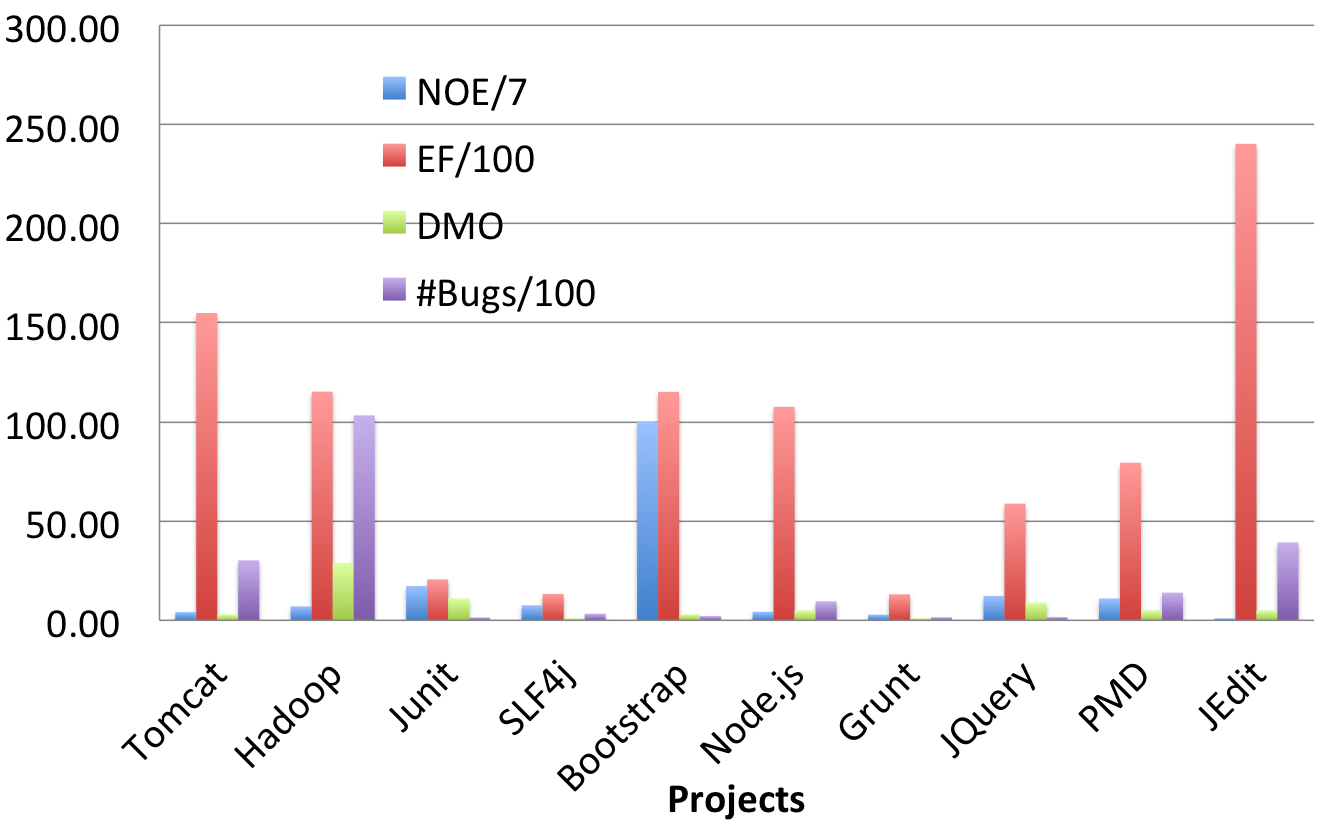
\includegraphics[scale=0.2]{figures/code-churn-metrics.png}
                    \caption{Repository Mining Tool Building}
                \end{figure}
        \end{frame}

    \subsection{Adoptability}
        \begin{frame}
            \frametitle{Adoptability}
            \textbf{Claim:}  Candoia apps are portable across diverse project settings and require no changes while adopting for new settings\\
            \textbf{Evaluation Strategy:}
            \begin{itemize}
                \item Implemted all 24 apps in Java for a project setting, keeping the tool modular and reusable
                \item Adopt the developed tool to new project setting
                \item Compared the LOC changes required in Candoia with Java to adopt a tool from a
                 project setting to another
            \end{itemize}
         \end{frame}

        \begin{frame}
            \frametitle{Project Settings Coverd by Test Projects}
            \begin{figure}[ht!] 
% \begin{footnotesize}
%\begin{scriptsize}
\centering
%\begin{minipage}{0.99\linewidth}
\begin{adjustbox}{max width=0.65\textwidth}
\begin{tabular}{|c|c|c|c|}
\hline
\rowcolor[HTML]{C0C0C0} 
\# & VCS & PL & Bugs \\
\hline\hline
1 & \inline{GIT} & \inline{Java} & \inline{Issues} \\ \hline
2 & \inline{SVN} & \inline{Java} & \inline{Bugzilla} \\ \hline
3 & \inline{GIT} & \inline{Java} & \inline{JIRA} \\ \hline
\end{tabular}
\end{adjustbox}
%\end{minipage}
%\begin{minipage}{0.99\linewidth}
\begin{adjustbox}{max width=0.65\textwidth}
\begin{tabular}{|c|c|c|c|}
\hline
\rowcolor[HTML]{C0C0C0} 
\# & VCS & PL & Bugs \\
\hline\hline
4 & \inline{GIT} & \inline{Java} & \inline{Tickets} \\ \hline
5 & \inline{SVN} & \inline{Java} & \inline{Tickets} \\ \hline
6 & \inline{GIT} & \inline{JS} & \inline{Issues} \\ \hline
\end{tabular}
\end{adjustbox}
%\end{minipage}
% \end{footnotesize}
%\end{scriptsize}
\caption{Six project settings}
\label{fig:project-settings}
\end{figure}
         \end{frame}

        \begin{frame}
            \frametitle{LOC changes in Boa v/s. Java}
            %\begin{figure*}
\begin{figure}
%\centering
%\resizebox{0.5\textwidth}{!}{%
\centering
\begin{adjustbox}{max width=\textwidth}
\begin{tabular}{|c|c|l|l|l|l|l|l|c|c|c|c|c|}
\hline
\rowcolor[HTML]{C0C0C0}
& \# & \multicolumn{6}{c}{Java} & \multicolumn{5}{c}{Candoia} \\ \hline
& & $M_{VCS}$ & $M_{Bug}$ & $M_{Forge}$ & $M_{Mining}$ & $M_{Visualize}$ &
\inline{Total} & \inline{Boa} & \inline{JS} & \inline{HTML} & \inline{CSS} &
\inline{Total} \\
\hline\hline

\multirow{6}{*}{\begin{sideways}Nullcheck\end{sideways}} 
& 1 & 125 & 157 & 20 & 143 & 53 & 498 & 59 & 12 & 34 & 0 & 105 \\ 
\cline{2-13} & 2 & 148 (-89,+112) & 117 (-119,+79) & 27 (-15,+22) & 156
(-43,+60) & 53 (-1,+1) & 501 (-267,+274) & 59 & 12 & 34 & 0 & 105 \\
\cline{2-13} & 3 & 125 (-2,+2) & 129 (-110,+82) & 20 (-1,+1) & 155 (-21,+33) &
53 (-1,+1) & 482 (-135,+118) & 59 & 12 & 34 & 0 & 105
\\
\cline{2-13} & 4 & 125 (-2,+2) & 115 (-111,+69) & 20 (-1,+1) & 167 (-18,+42) &
53 (-1,+1) & 480 (-133,+115) & 59 & 12 & 34 & 0 & 105
\\
\cline{2-13} & 5 & 148 (-89,+112) & 116 (-110,+69) & 27 (-15,+22) & 154
(-48,+59) & 53 (-1,+1) & 498 (-263,+263) & 59 & 12 & 34 & 0 & 105
\\
\cline{2-13} & 6 & 120 (-15,+10) & 157 (-1,+1) & 20 (-1,+1) & 147 (-13,+17) &
53 (-1,+1) & 497 (-31,+30) & 59 & 12 & 34 & 0 & 105
\\
\hline

\multirow{6}{*}{\begin{sideways}File Association\end{sideways}}
& 1 & 72 & 139 & 20 & 138 & 53 & 422 & 20 & 12 & 34 & 0 & 66 \\ 
\cline{2-13} & 2 & 125 (-38,+91) & 60 (-113,+34) & 27 (-15,+22) & 140 (-45,+47)
& 53 (-1,+1) & 405 (-212,+195) & 20 & 12 & 34 & 0 & 66 \\
\cline{2-13} & 3 & 72 (-1,+1) & 146 (-120,+127) & 20 (-1,+1) & 146 (-7,+15) & 53
(-1,+1) & 437 (-130,+145) & 20 & 12 & 34 & 0 & 66 \\ 
\cline{2-13} & 4 & 72 (-1,+1) & 115 (-106,+72) & 20 (-1,+1) & 137 (-4,+3) & 53
(-1,+1) & 397 (-113,+78) & 20 & 12 & 34 & 0 & 66 \\
\cline{2-13} & 5 & 125 (-38,+91) & 95 (-96,+52) & 27 (-15,+22) & 133 (-30,+25) &
53 (-1,+1) & 433 (-180,+191) & 20 & 12 & 34 & 0 & 66 \\
\cline{2-13} & 6 & 72 (-1,+1) & 139 (-1,+1) & 20 (-1,+1) & 138 (-1,+1) & 53
(-1,+1) & 421 (-5,+5) & 20 & 12 & 34 & 0 & 66 \\ \hline

\multirow{6}{*}{\begin{sideways}Churn Rate\end{sideways}}  
& 1 & 52 & 0 & 20 & 69 & 53 & 194 & 13 & 33 & 47 & 0 & 93 \\ 

\cline{2-13} & 2 & 104 (-38,+90) & 0 & 27 (-15,+22) & 74 (-26,+31) & 53 (-1,+1)
& 258 (-80,+144) & 13 & 33 & 47 & 0 & 93 \\

\cline{2-13} & 3 & 52 & 0 & 20 (-1,+1) & 69 & 53 (-1,+1) & 194 (-2,+2) & 13 & 33 & 47 & 0 & 93 \\ 

\cline{2-13} & 4 & 52 & 0 & 20 (-1,+1) & 69 & 53 (-1,+1) & 194 (-2,+2) & 13 & 33 & 47 & 0 & 93 \\

\cline{2-13} & 5 & 104 (-38,+90) & 0 & 27 (-15,+22) & 74 (-26,+31) & 53 (-1,+1)
& 258 (-80,+144) & 13 & 33 & 47 & 0 & 93 \\

\cline{2-13} & 6 & 52 & 0 & 20 (-1,+1) & 69 & 53 (-1,+1) & 194 (-2,+2)
& 13 & 33 & 47 & 0 & 93 \\ \hline

\multirow{6}{*}{\begin{sideways}BugSrc Mapper\end{sideways}}
& 1 & 78 & 152 & 20 & 73 & 53 & 376 & 37 & 30 & 47 & 32 & 146 \\ 

\cline{2-13} & 2 & 105 (-49,+76) & 79 (-118,+45) & 27 (-15,+22) & 74 (-41,+42) &
53 (-1,+1) & 338 (-224,+186) & 37 & 30 & 47 & 32 & 146 \\

\cline{2-13} & 3 & 78 (-2,+2) & 104 (-111,+63) & 20 (-1,+1) & 78 (-28,+33) & 53
(-1,+1) & 333 (-143,+100) & 37 & 30 & 47 & 32 & 146 \\

\cline{2-13} & 4 & 78 (-2,+2) & 85 (-106,+39) & 20 (-1,+1) & 77 (-24,+28) & 53
(-1,+1) & 313 (-134,+71) & 37 & 30 & 47 & 32 & 146 \\

\cline{2-13} & 5 & 108 (-44,+74) & 85 (-106,+39) & 27 (-15,+22) & 69 (-45,+41) &
53 (-1,+1) & 342 (-211,+177) & 37 & 30 & 47 & 32 & 146 \\

\cline{2-13} & 6 & 78 (-2,+2) & 152 (-1,+1) & 20 (-1,+1) & 78 (-28,+33) & 53
(-1,+1) & 381 (-33,+38) & 37 & 30 & 47 & 32 & 146 \\
\hline

% \multirow{6}{*}{\begin{sideways}Method Usage\end{sideways}}
% & 1 & a & b & c & d & e & f & p & q & r & s & t \\ \cline{2-13}
% & 2 & a & b & c & d & e & f & p & q & r & s & t \\ \cline{2-13}
% & 3 & a & b & c & d & e & f & p & q & r & s & t \\ \cline{2-13}
% & 4 & a & b & c & d & e & f & p & q & r & s & t \\ \cline{2-13}
% & 5 & a & b & c & d & e & f & p & q & r & s & t \\ \cline{2-13}
% & 6 & a & b & c & d & e & f & p & q & r & s & t \\ \hline
\end{tabular}
\end{adjustbox}
\caption{\tiny{Compares LOC changes required for adopting apps from one project
setting to another in Java and Candoia.}}
\label{fig:adoptability}
%}
%\end{figure*}
\end{figure}
         \end{frame}

 \subsection{Customizability}
        \begin{frame}
            \frametitle{Customizability}
            \textbf{Claim:} Performing customizations in Candoia requires less efforts in terms of LOC \\
            \textbf{Evaluation Criteria:}
            \begin{itemize}
                \item Customize the Java and Candoia apps
                \item Customizations include change in Mining logic, visualization, external tool usage etc.
                \item Compared the LOC changes required to customize the Candoia app with Java tool
            \end{itemize}
         \end{frame}

        \begin{frame}
%            \frametitle{LOC changes in Boa v/s. Java}
            \begin{figure}
\centering
\begin{scriptsize}
\begin{adjustbox}{max width=\textwidth}
\begin{tabular}{|c|c||c|c|}
\hline
$c_{10}$ & Shows number of nullcheck bug revisions in pie chart & $c_{23}$ &
Module association instead of file association \\
\hline 

$c_{11}$ & Change the output display to column chart & $c_{24}$ & File
association without bug data \\
\hline

$c_{12}$ & Display nullcheck issue life time & $c_{30}$ & Churn rate based on
revisions \\
\hline

$c_{13}$ & Plot nullcheck date v/s number of modified files & $c_{31}$ &
Associate bugs to churn rates \\
\hline 

$c_{14}$ & Maps nullcheck to developers & $c_{40}$ & Bugs to source files
mapping displayed in column chart \\
\hline

$c_{20}$ & File associations using weka apriori & $c_{41}$ & Change the output
display to pie chart \\
\hline

$c_{21}$ & File associations using weka fpgrowth & $c_{42}$ & Top five files
with maximum bug fix time \\
\hline

$c_{22}$ & File associations using spmf eclat & $c_{43}$ & Asssociate
developers to bugs \\
\hline
\end{tabular}
\end{adjustbox}
\end{scriptsize}

\begin{adjustbox}{max width=\textwidth}
\begin{tabular}{|c|c|l|l|l|l|l|l|l|l|l|l|l|}
\hline
\rowcolor[HTML]{C0C0C0}
& \# & \multicolumn{6}{c}{Java} & \multicolumn{5}{|c}{Candoia{}} \\ \hline
& & $M_{VCS}$ & $M_{Bug}$ & $M_{Forge}$ & $M_{Mining}$ & $
M_{Visualize}$ & \inline{Total} & \inline{Boa} & \inline{JS} & \inline{HTML} &
\inline{CSS} & \inline{Total} \\
\hline\hline

\multirow{5}{*}{\begin{sideways}Nullcheck\end{sideways}} 
& $c_{10}$ & 125 & 157 & 20 & 143 & 53 & 498 & 59 & 41 & 45 & 26 & 171 \\ 

\cline{2-13} & $c_{11}$ & 125 (-1,+1) & 157 (-1,+1) & 20 (-1,+1) & 143 (-2,+2) &
53 (-3,+3) & 498 (-8,+8) & 59 & 12 & 34 & 0 & 105
\\

\cline{2-13} & $c_{12}$ & 125 (-1,+1) & 137 (-29,+9) & 20 (-1,+1) & 144
(-14,+11) & 53 (-2,+2) & 479 (-47,+24) & 74 (-4,+19) & 41 (-2,+2) & 45 (-4,+4) &
26 (-1,+1) & 186 (-11,+26)
\\

\cline{2-13} & $c_{13}$ & 125 (-1,+1) & 157 (-1,+1) & 20 (-1,+1) & 147 (-6,+11)
& 53 (-1,+1) & 501 (-10,+15) & 64 (-3,+8) & 41 (-4,+4) & 45 (-4,+4) & 26 (-1,+1)
& 176 (-12,+17)
\\

\cline{2-13} & $c_{14}$ & 125 (-1,+1) & 157 (-1,+1) & 20 (-1,+1) & 147 (-13,+18)
& 53 (-1,+1) & 502 (-17,+22) & 61 (-4,+1) & 41 (-4,+4) & 45 (-4,+4) & 26 (-1,+1)
& 173 (-13,+10)
\\

\hline

\multirow{5}{*}{\begin{sideways}File Assoc.\end{sideways}} 
& $c_{20}$ & 141 & 157 & 20 & 178 & 23 & 481 & 37 & 12 & 34 & 0 & 83 \\
 
\cline{2-13} & $c_{21}$ & 141 (-1,+1) & 157 (-1,+1) & 20 (-1,+1) & 178 (-3,+3) &
23 (-1,+1) & 481 (-7,+7) & 37 & 12 (-1,+1) & 34 & 0 & 83 (-1,+1)
\\

\cline{2-13} & $c_{22}$ & 141 (-1,+1) & 157 (-1,+1) & 20 (-1,+1) & 183 (-23,+28)
& 23 (-1,+1) & 486 (-27,+32) & 37 & 12 (-1,+1) & 34 & 0 & 83 (-1,+1)
\\

\cline{2-13} & $c_{23}$ & 141 (-1,+1) & 157 (-1,+1) & 20 (-1,+1) & 178 (-3,+3) &
23 (-1,+1) & 461 (-8,+34) & 37 & 12 (-1,+1) & 34 & 0 & 83 (-1,+1)
\\

\cline{2-13} & $c_{24}$ & 141 (-1,+1) & 0 & 20 (-1,+1) & 175 (-5,+2) & 23
(-1,+1) & 359 (-165,+5) & 24 (-20,+7) & 12 (-1,+1) & 34 & 0 & 70 (-21,+8)
\\

\hline

\multirow{2}{*}{\begin{sideways}Churn\end{sideways}} 
& $c_{30}$ & 52 & 0 & 20 & 69 & 53 & 194 & 13 & 33 & 47 & 0 & 93 \\ 

\cline{2-13} & $c_{31}$ & 72 (-1,+21) & 0 & 20 (-1,+1) & 73 (-4,+8) & 53 (-1,+1)
& 218 (-7,+31) & 42 (-4,33) & 33 & 47 & 0 & 122 (-4,+33)
\\

\hline

\multirow{4}{*}{\begin{sideways}BugSrc\end{sideways}} 
& $c_{40}$ & 78 & 152 & 20 & 73 & 53 & 376 & 37 & 30 & 47 & 32 & 146 \\ 

\cline{2-13} & $c_{41}$ & 78 (-2,+2) & 152 (-2,+2) & 20 (-1,+1) & 73 (-1,+1) &
53 (-2,+2) & 376 (-8,+8) & 37 & 38 (-28,+35) & 47 & 32 & 154 (-28,+35)
\\

\cline{2-13} & $c_{42}$ & 78 (-2,+2) & 152 (-2,+2) & 20 (-1,+1) & 137 (-18,+82)
& 53 (-1,+1) & 440 (-24,+88) & 41 (-15,+19) & 30 & 47 & 32 & 155 (-15,+19)
\\
  
\cline{2-13} & $c_{43}$ & 78 (-2,+2) & 157 (-17,+23) & 20 (-1,+1) & 99 (-19,+47)
& 53 (-1,+1) & 407 (-40,+74) & 46 (-2,+11) & 38 (-4,+12) & 47 & 32 & 163
(-6,+23)
\\

\hline
\end{tabular}
\end{adjustbox}
\caption{\tiny{Compares LOC changes required for a number of customizations in Java and Candoia.}}
\label{fig:customizability}
\end{figure}
         \end{frame}